%!TEX root = *.tex
%%%%%%%%%%%%%%%%%%
% カウンタのリセット
\setcounter{figure}{0}
% 問題文
{
\begin{wrapfigure}{r}{16zw}
  \vspace{-\intextsep}
  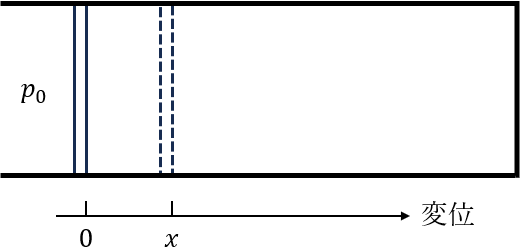
\includegraphics[width=16zw]{../graphs/se_1H_120.png}
\end{wrapfigure}
図のようにピストンを持つ気密なシリンダーを水平に保ち,
内部に比熱比$\gamma$の理想気体を入れて圧力$p_0$の大気中に置いた.
ピストンのつりあいの位置を$x=0$とし,
ピストンの質量と底面積をそれぞれ$m,\,S$とする.
またこのときのシリンダー内の気体の体積を$V_0$とする.
気体定数を$R$,ピストンとシリンダー間の摩擦は無視できるとして以下の問いに答えよ.
$\abs{z}\ll 1$の場合,近似式$(1+z)^\alpha \fallingdotseq 1+\alpha z$を用いよ.

\par}
\begin{enumerate}[(1)]
  \setlength{\leftskip}{-1.5zw}
  \setlength{\itemindent}{1zw}\setlength{\labelsep}{0.5zw}
  \setlength{\labelwidth}{1zw}\setlength{\leftmargin}{1zw}
  \setlength{\itemsep}{0.5\baselineskip}
  \item 気体の温度を一定に保ったままピストンを\x だけ押した.
  このときのシリンダー内の気体の圧力$p_x$を求めよ.
  押したときのピストンの位置は図中に点線で示してある.
  ただし,$\abs{x}\leqq a\ll V_0/S$とする.
  \item 時刻$t=0$において微小変位$x=a\,(>0)$からピストンを放したところ,
  ピストンは往復運動を始めた.
  シリンダー内の気体の温度が一定に保たれているとして,
  周期$T$を求め,\x を$t$の関数として表せ.
  \item シリンダー内の気体への熱の出入りがないとしたとき,
  (2)の場合(温度が一定)に比べてピストンの往復運動の周期は何倍になるか.
\end{enumerate}




% メモ
\begin{comment}

\end{comment}


%%%%%%%%%%%%%%%%%%